\section{Visual Snow}

Visual snow offers a unique window into how ECC's framework can explain perceptual phenomena that challenge traditional computational models of consciousness. This condition, characterized by continuous visual static perceived across the entire visual field \cite{Puledda2020}, provides compelling evidence for how consciousness emerges from and remains grounded in underlying patterns of energetic coherence.

The phenomenon demonstrates several key principles of ECC's framework. Unlike typical visual processing, which involves organized patterns of neural activity representing external stimuli, visual snow appears to reveal the background energy dynamics that typically remain below the threshold of conscious awareness. This aligns with evidence suggesting that visual snow may represent a fundamental dysrhythmia in thalamocortical circuits \cite{Lauschke2016}, affecting how the brain maintains coherent visual representations.

Recent clinical investigations have established visual snow as a distinct neurological condition rather than merely a symptom of other disorders \cite{Schankin2014}. The persistence of visual static across different lighting conditions and its independence from external stimuli suggest that it emerges from alterations in how the brain maintains coherent visual states rather than from disruptions in early sensory processing \cite{Bessero2014}.

Through ECC's framework, visual snow can be understood as a modification in how the brain achieves and maintains coherent energy states in visual processing regions. The continuous, grainy quality of the phenomenon reflects underlying patterns of energetic activity that normally remain integrated into seamless visual experience. This interpretation aligns with predictive processing accounts of perception \cite{Clark2013}, suggesting that visual snow represents a disruption in how the brain maintains stable perceptual predictions through coherent energy dynamics.

The relationship between visual snow and other perceptual phenomena becomes particularly clear through ECC's emphasis on energetic coherence. The frequent co-occurrence of persistent after-images and enhanced pattern sensitivity in visual snow patients \cite{Puledda2020} suggests broader alterations in how visual processing regions maintain coherent states. These associated symptoms indicate that visual snow involves fundamental changes in how the brain organizes visual experience through patterns of energetic coherence rather than simple sensory disruption.

This understanding has important implications for both theoretical models of consciousness and clinical approaches to visual snow. Rather than treating the condition as a processing error or pathological activation, ECC suggests it represents an alternative configuration of how consciousness organizes visual experience through energetic coherence. This perspective aligns with embodied approaches to perception \cite{ORegan2001} while providing a specific mechanism - disrupted patterns of energetic coherence - through which altered visual experiences can emerge.

The framework also suggests why visual snow proves resistant to traditional treatments targeting neurotransmitter systems. If the condition represents a fundamental reorganization of how visual regions maintain coherent states, interventions (should they even be required or desired) may need to focus on restoring appropriate patterns of energetic coherence rather than simply modulating neural activity. This understanding could guide the development of new therapeutic approaches based on supporting stable patterns of visual coherence.

Visual snow thus serves as a crucial test case for understanding how consciousness emerges from patterns of energetic coherence in neural systems. The condition demonstrates both the flexibility and constraints of conscious visual processing while suggesting new approaches to investigating and treating disorders of perceptual organization.

\begin{figure}[h]
    \centering
    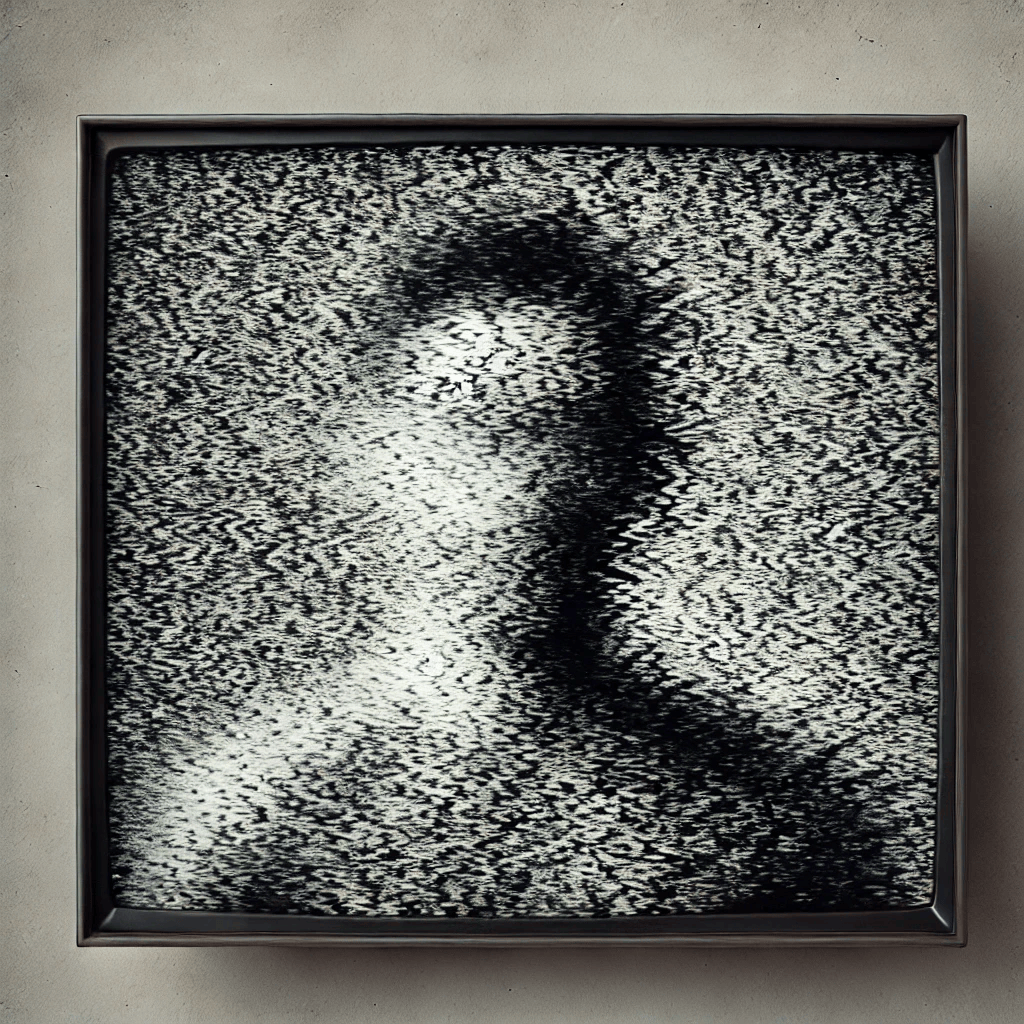
\includegraphics[width=0.8\textwidth]{snow.png}

    \caption{An exaggerated depiction of visual snow.}
\end{figure}

Building on this foundation, we can further explore how visual snow illuminates fundamental principles of perceptual organization through the lens of energetic coherence. Traditional predictive coding accounts \cite{Rao1999, Friston2009} suggest that perception emerges from hierarchical prediction processes, but ECC extends this understanding by grounding these processes in patterns of energetic coherence that maintain stable perceptual states.

The phenomenology of visual snow provides crucial insights into how consciousness maintains coherent perceptual fields. Rather than representing random noise in visual processing, the consistent and organized nature of visual snow - its characteristic density, temporal dynamics, and field-like distribution - suggests disruption in how the brain maintains background patterns of energetic coherence. This aligns with enactive approaches to perception \cite{Varela1991} while providing specific mechanisms through which perceptual experiences emerge from neural dynamics.

Recent theoretical work in sensorimotor contingencies \cite{Seth2014} helps explain why visual snow remains relatively stable across different viewing conditions and contexts. Unlike hallucinations or other visual phenomena that vary with attention or environmental conditions, visual snow maintains consistent characteristics that suggest fundamental alterations in how visual consciousness achieves coherent organization. This stability points to changes in the underlying energetic patterns that support visual experience rather than disruptions in higher-level processing.

The relationship between visual snow and broader theories of consciousness becomes particularly clear when considering how the condition affects perceptual presence - the sense that perceived objects are real and present in the environment \cite{Seth2014}. While visual snow patients maintain normal perception of external objects, the constant presence of visual static reveals how consciousness simultaneously maintains multiple layers of perceptual organization through distinct patterns of energetic coherence.

This multi-level organization of visual consciousness aligns with philosophical accounts of perception that emphasize its active, constitutive nature \cite{Noe2004}. Visual snow demonstrates how consciousness doesn't simply process sensory inputs but actively maintains coherent perceptual states through sophisticated patterns of energetic organization. The condition reveals these organizational processes by making typically implicit aspects of visual processing explicitly present in consciousness.

The theoretical significance of visual snow extends beyond clinical understanding to fundamental questions about the nature of conscious perception. The condition challenges purely representational theories of consciousness \cite{Metzinger2003} by demonstrating how perceptual experience emerges from and remains grounded in patterns of energetic coherence rather than abstract information processing. This suggests new approaches to investigating both normal perception and its alterations in various conditions.

The relationship between visual snow and other perceptual variations provides deeper insight into how consciousness maintains coherent visual states through patterns of energetic organization. Much like color perception demonstrates structured relationships that resist arbitrary reconfiguration \cite{Palmer1999}, visual snow reveals fundamental aspects of how visual consciousness achieves stable organization through coherent energy dynamics.

This perspective aligns with research suggesting that perception emerges from structured relationships within neural systems rather than arbitrary mappings between stimuli and experience \cite{Thompson1995}. Visual snow demonstrates how these relationships can be systematically altered while maintaining basic coherence - the visual static remains organized and stable even as it modifies normal visual experience. This structured modification suggests that consciousness operates through constrained patterns of energetic coherence rather than through unconstrained information processing.

The condition also illuminates debates about the plasticity of perceptual categories \cite{VanBrakel1993}. While visual snow represents a dramatic alteration in visual experience, it maintains consistent characteristics across individuals and contexts, suggesting fundamental constraints on how consciousness can organize visual experience through patterns of energetic coherence. These constraints help explain both the stability of normal perception and the specific ways it can be altered in various conditions.

Understanding visual snow through ECC's framework provides new perspective on classical problems in philosophy of perception, such as the relationship between subjective experience and neural activity \cite{Tye2000}. Rather than requiring a solution to the hard problem of consciousness, ECC suggests that visual snow reveals how conscious experience emerges directly from patterns of energetic coherence in neural systems. This helps explain both the phenomenal character of visual snow and its resistance to reduction to purely computational descriptions.

The implications extend beyond theoretical understanding to practical approaches for investigating and treating perceptual disorders. By recognizing how visual snow emerges from altered patterns of energetic coherence rather than simple processing disruptions, researchers and clinicians might develop more effective interventions focused on restoring appropriate patterns of perceptual organization. This could lead to novel therapeutic approaches that target the underlying organizational principles of visual consciousness rather than just its surface manifestations.

Visual snow thus serves as a crucial case study for understanding how consciousness emerges from and maintains coherent perceptual states through sophisticated patterns of energetic organization. The condition reveals fundamental principles about how consciousness operates while suggesting new directions for both theoretical research and clinical practice. This understanding helps bridge the gap between subjective experience and neural dynamics while providing concrete approaches to investigating and treating disorders of conscious perception.